\Subsection{Naive payment network}
The current form of our payment channel works very well as long as it is between just two parties. A very helpful feature would be to be able to send money to anyone without having a direct channel between you and that person, in other word the transaction jumps between any number of other channels before reaching it's destination. If we naively use the channel we have constructed in the previous section as is to send money over multiple jumps we would run into the following problem:

Imagine there being 3 people: Alice (A), Bob (B) and Cecil (C). Alice and Bob have a channel between each other and Bob and Cecil have a channel between each other. Making the following graph: A - B - C. Alice wants to send money to Cecil but they have no channel between each other. To solve this Alice asks Bob to promise to send x amount of money to Cecil if Alice sends x amount of money to Bob. In the perfect world Bob would be honest and this system of payment networking would work. In the real world however having to trust every node between you and the destination would cause problems with malicious nodes. There is nothing stopping Bob from taking Alice's money and never sending anything to Cecil. 

The channel has to be extended further to allow multi-hop payments and still retain it's breach remedy feature. This is where Hashed Time Locked Contracts come into the picture. 

\Subsection{Payment channels with Hashed Time Locked Contracts}
A new mechanism needs to be added to our payment channel to enforce that multi-hop transactions actually make it all the way to their destination while at the same time still retaining the breach remedy mechanism etc... 

This could be done by adding a third output to the commitment transactions. This new output pays to a hashed time locked contract (\textbf{HTLC}).\cite{antonopoulos_2017}\cite{lightningnetwork_2019} Before when a payment was made over a payment channel the amount was updated for each output representing a user in the channel. With the HTLC-output the amount sent is represented by the the value of the HTLC-output.\cite{lightningnetwork_2019}\cite{bolt}

A channel could be thought of as having three states: regular, unsettled, and settled. The regular state is the one described in previous sections, it's a channel with one set of active commits, the commit will not have any HTLC-outputs.\cite{lightningnetwork_2019} A channel where the latest commits has a HTLC-output is considered unsettled. The unsettled state should only exists while there is uncertainty about whether the multi-hop transaction completed or not. You could say that \textbf{the HTLC-output only exists as a contingency}, if both parties cooperate the channel can return to regular state with the channel balances updated accordingly, if the parties cannot agree or for some reason will not cooperate the channel should be close as soon as possible, as to why we will get to that.\cite{lightningnetwork_2019} A channel reaches a settled state when both parties decides to close the channel, it is done by creating one last pair of commitment transactions but without any revocable deliveries. After a channel is settled no further transactions could be exchanged in it safely as the mechanism for preventing old transactions from being broadcast has been removed, instead the commitment transaction should be broadcast and the channel properly closed.\cite{lightningnetwork_2019}\cite{bolt}

To understand the HTLC-output you first need to understand the general mechanism that is used to ensure that multi-hop transactions work. 

\begin{figure}[H]
	\centering
	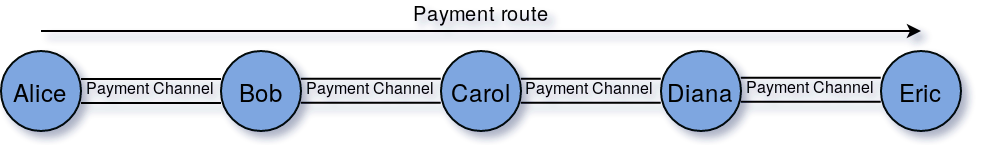
\includegraphics[width=1\textwidth]{background/images/ln_route.png}
	\caption{An overview of a network formed by payment channels}
	\label{fig:pc-route}
\end{figure}

The principle used for multi-hop transactions is a lot like the one used for on-chain atomic swaps. It relies on revealing a secret pre-image\footnote{See glossary} of a hash within a certain time limit. Using the diagram in figure \ref{fig:pc-route} as example. Alice wants to send money to Eric. But they have no direct channel between each other. To make this work Alice asks Eric for a hash of a secret, let's call this $H = SHA256(R)$. For now Eric holds on to R and only sends H to Alice.

For the money to reach Eric, Alice needs to go via Bob. To do this Alice requests from Bob that they make a new commitment transaction with one HTLC output. The amount in the output should be equal to to whatever amount Alice want to send to Eric. The promise here is that Bob will get this money only if he can prove that he has the pre-image to H. Bob does the same with Carol. This continues until an updated commitment reaches Eric. Eric can then send the pre-image R backwards through the chain until it reaches Alice. 

\begin{figure}[H]
	\centering
	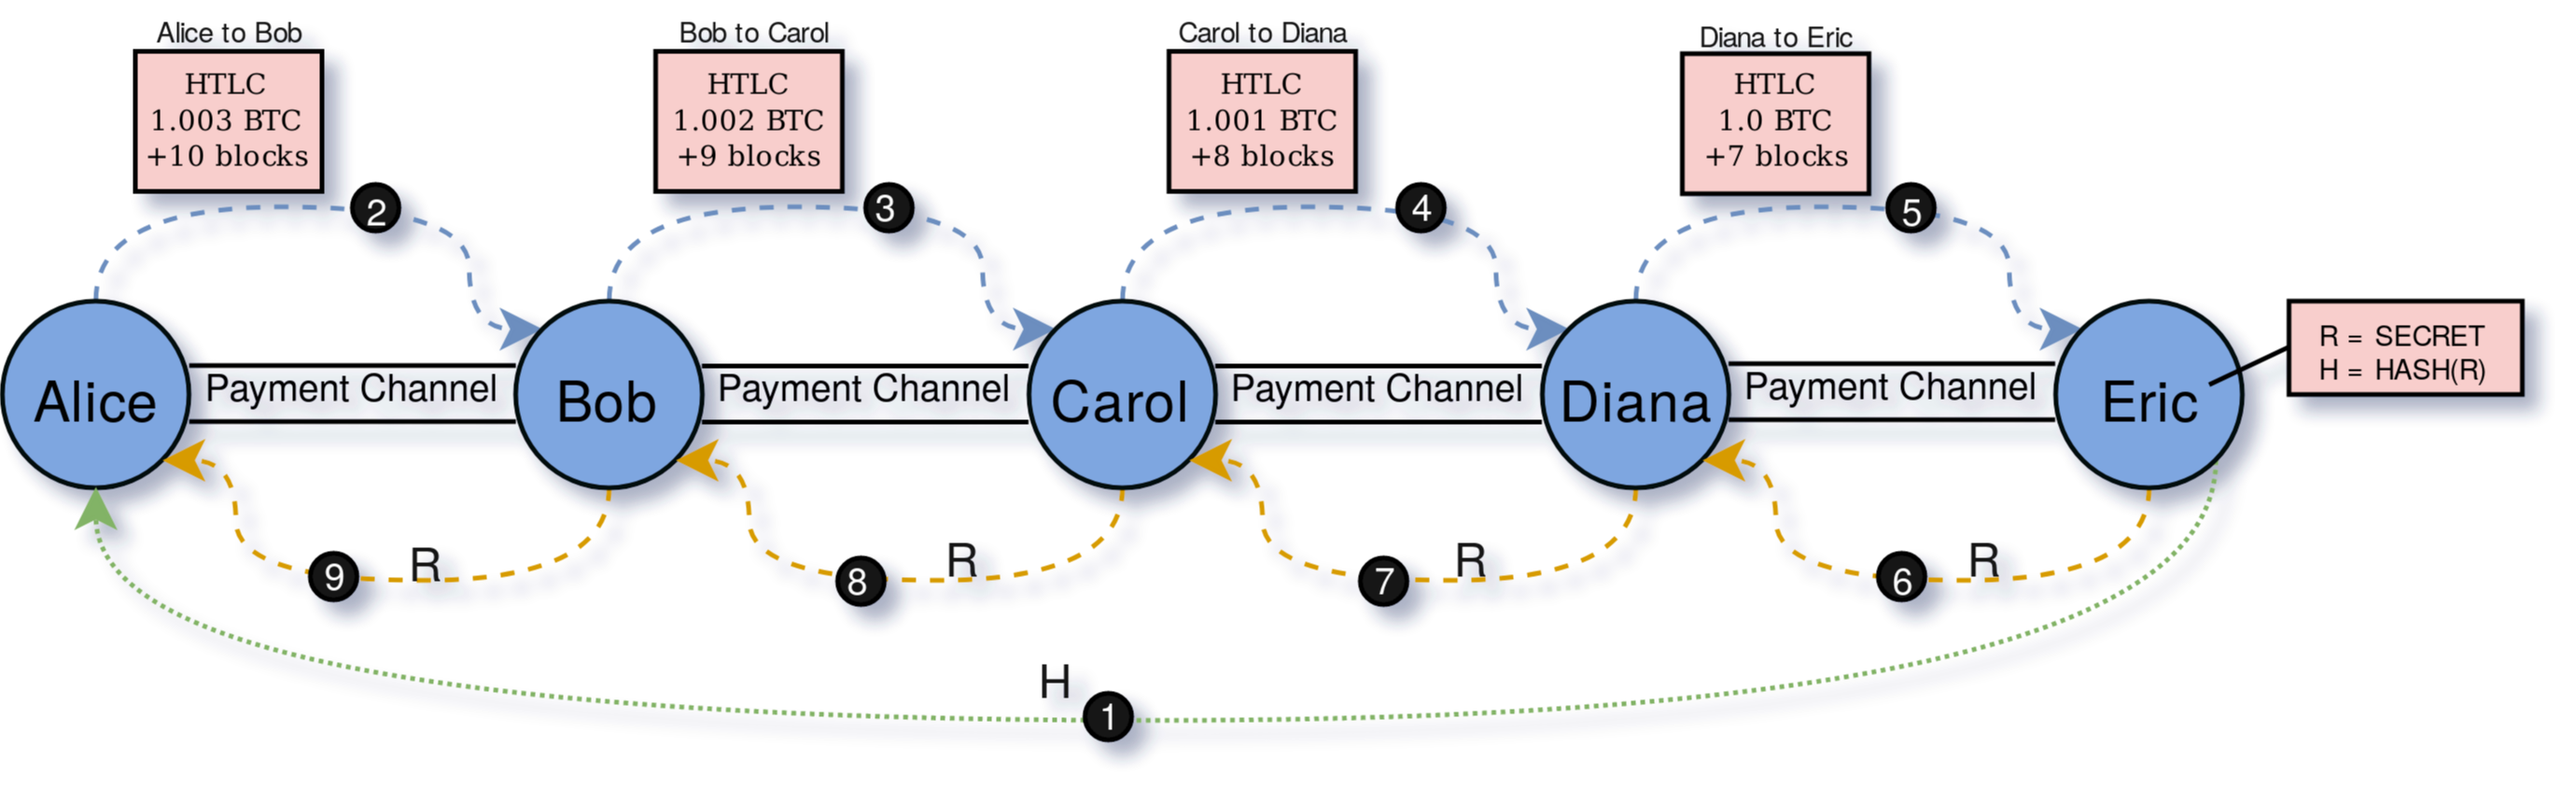
\includegraphics[width=1.1\textwidth]{background/images/ln_route_htlc.png}
	\caption{All the steps taken in the payment network}
	\label{fig:pc-route-final}
\end{figure}

Earlier it was mentioned that the HTLC output only existed as a contingency, when Bob can prove to Alice that he knows the pre-image R, and can claim the money in the htlc-output by closing the channel, Alice has no reason to not update the channel with correct balances in Bob's favor. Thus the channel returns to a regular state with no htlc-outputs and all previous commits are revoked. This is done for all channels between Alice and Eric. If a party will not co-operate in the chain the channels to that person will have to be closed, this is the only case where the htlc-outputs are actually spent. There is no risk of monetary loss, closing channels is generally something that should be avoided if not absolutely necessary.

\Subsection{HTLC in more detail}
The HTLC script is a bit different depending on what side you are on in the channel, in other words the HTLC in the commitment of the sender is different to the one on the receiver end. What they both have in common however is the three possible outcomes. Let's call these paths \textbf{HTLC timeout}, \textbf{HTLC execution} and \textbf{HTLC breach remedy}.

HTLC execution can be considered to be the main path and the one that is taken if everything goes as planned. Let's take a closer look at what happens in the channel between Alice and Bob in figure \ref{fig:pc-route-final}. Bob knows the secret R because Carol sent it to him. Under normal circumstances Bob would prove to Alice that he knows the secret R, Alice would accept and the channel would be updated to reflect the transaction taking place. But for the sake of example let's say that Alice is uncooperative and does not want to give up the money she just sent to Eric. 
Bob should then close the channel with Alice and claim his money in the HTLC output by providing a input containing the pre-image (R) and required signatures.

HTLC timeout is the path taken in the case where Bob never received the pre-image (R) from Carol. In this case the money should be refunded to Alice. Under normal circumstance Bob sees that Alice can claim the money and thus updates the channel to reflect the refund. In the case where Bob refuses to cooperate Alice can close the channel after the timeout has passed. This time no pre-mage is needed, only the signatures from both channel parties.

HTLC breach remedy pays the money directly to the party that did not send an old commitment transaction. The breach remedy path is redeemed by providing a correct signature with the revocation key.

The second-level HTLC is a necessary second part of the HTLC output. Whenever a HTLC-output is spent by the same person that broadcast their commitment transaction it has to lead into a second-level HTLC script, this is enforced by the HTLC script requiring the signature from both parties depending on what side of the commitment tree you are on. The second-level HTLC script is fairly basic, it has two outcomes. Either the spender has to wait x amount of blocks (in relative time) before spending, or it can be revoked immidietly if a signature with the revocation keys is provided. Its usefulness can be demonstrated with an example:

Take the example where a transaction from Alice to Eric passed through a channel between Alice and Bob. Let's say a couple of days passed and Alice and Bob has exchanged other transactions since. Without second level HTLC Bob could broadcast the old commitment transaction and try to claim the HTLC-output money by providing the pre-image. With second-level HTLC Bob needs to wait a relative time before the money properly becomes his. If the old commit was properly revoked Alice could revoke Bob's attempt at claiming the HTLC-ouput. Same holds true the other way around if Alice tries to claim an old HTLC output by waiting for the timeout.

Figure \ref{fig:pc-htlc} is the equivalent transaction flow diagram for a channel where the third commit contains a HTLC-output. \textbf{To keep the diagram from exploding completely all the previous and following commitment transactions has been excluded.} Also included are all the revocations, so it can be assumed that other commitments were made on this channel after this one.  

\begin{figure}[H]
	\centering
	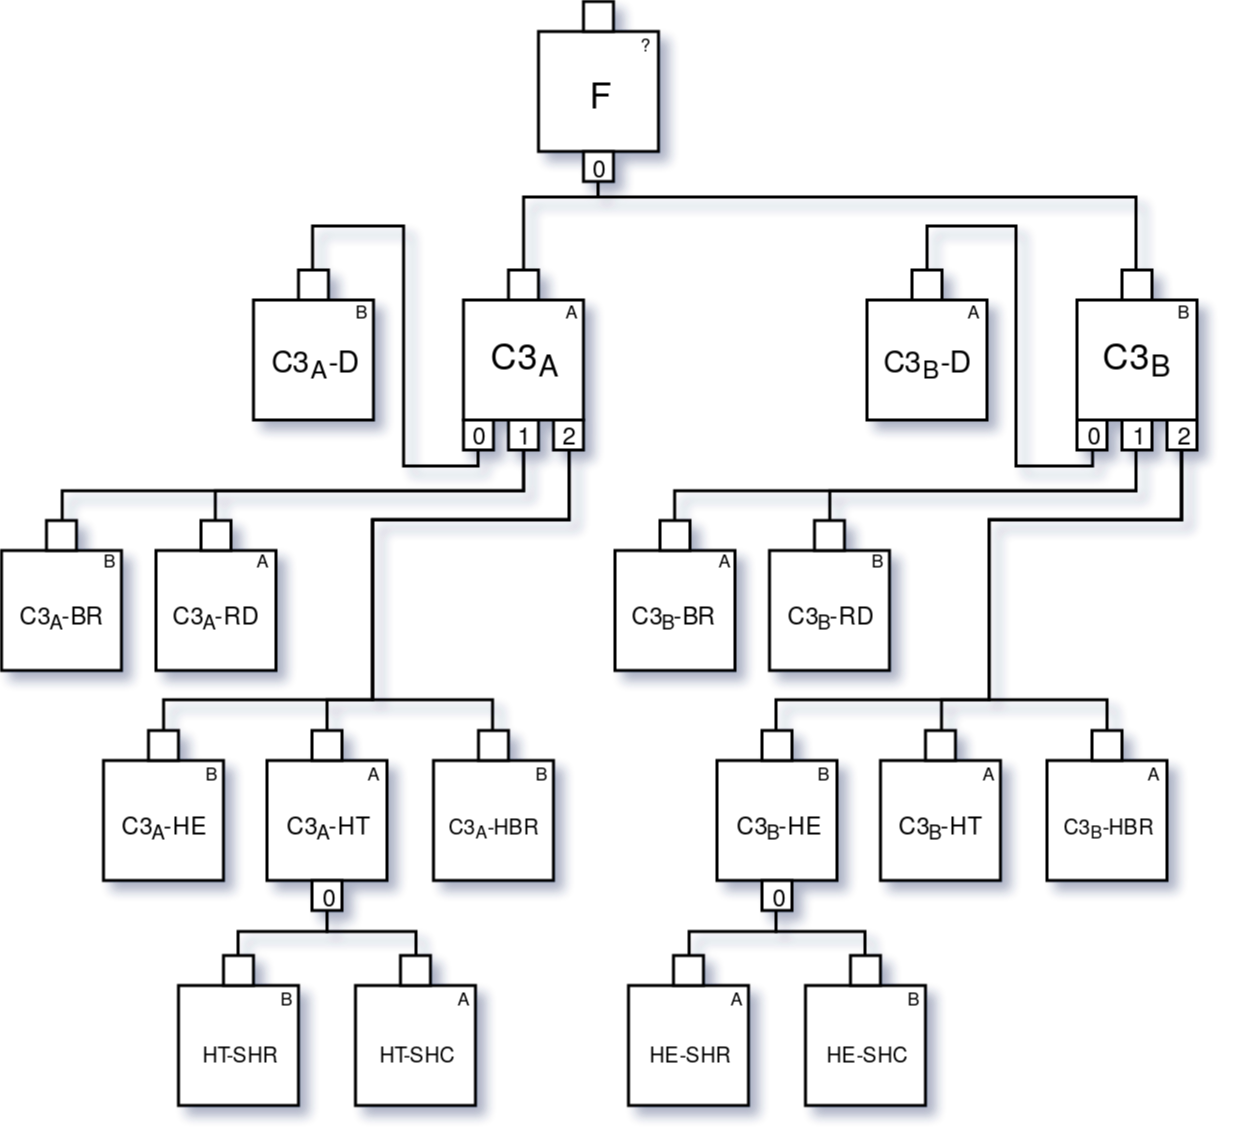
\includegraphics[width=0.80\textwidth]{background/images/payment_channel_htlc.png}
	\caption{The transaction diagram showing the htlc-outputs this time. In the diagram Alice (A) is the sender and Bob (B) is the receiver}
	\label{fig:pc-htlc}
\end{figure}

\begin{figure}[H]
	\centering
	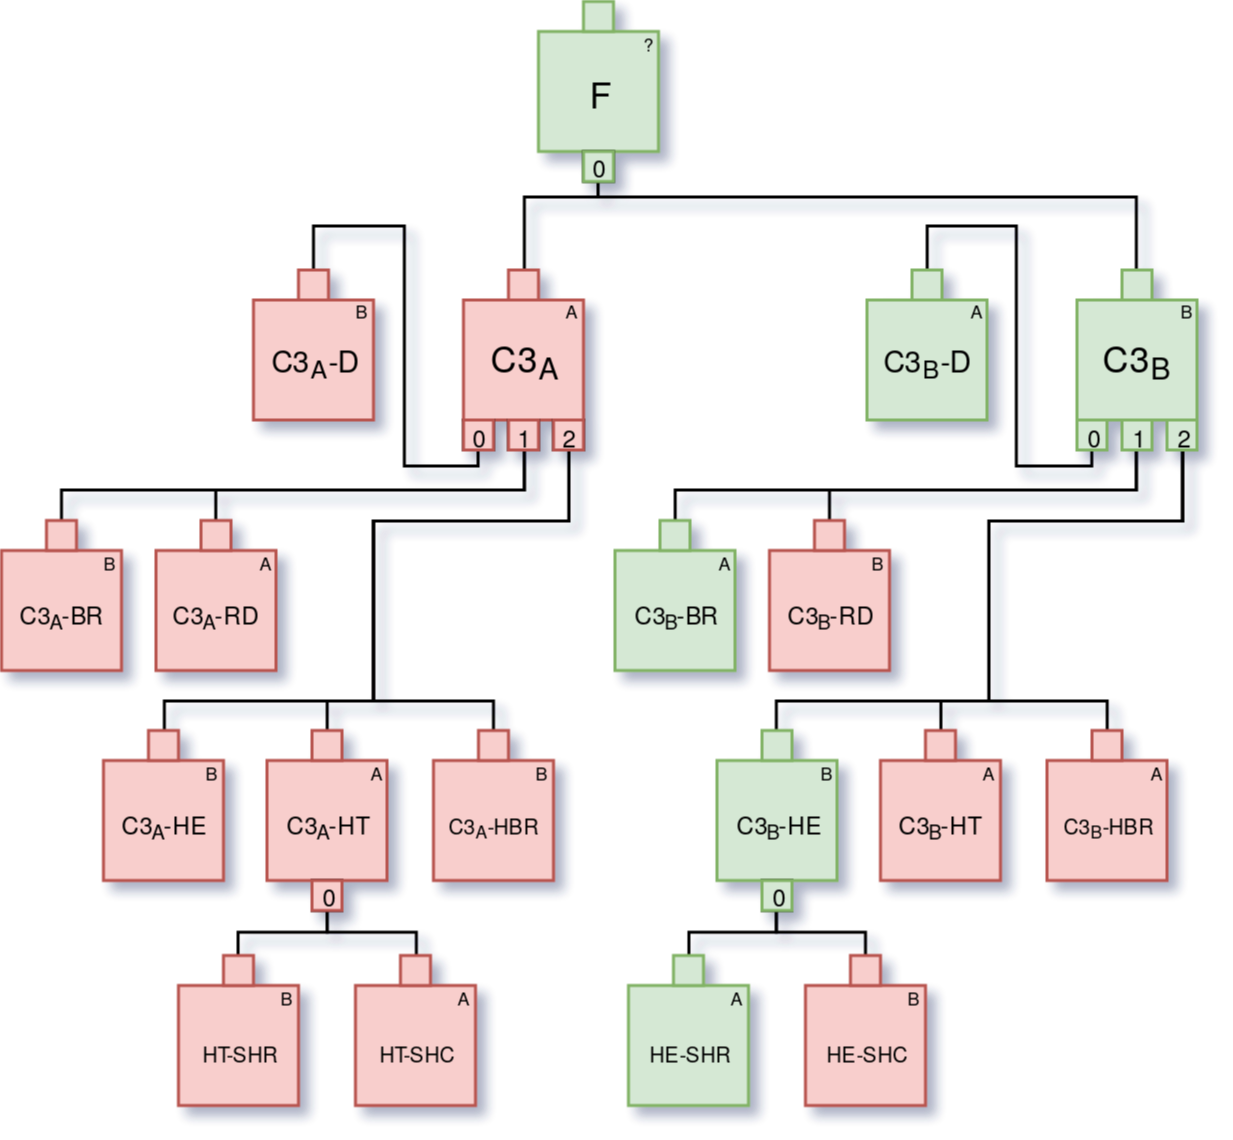
\includegraphics[width=0.80\textwidth]{background/images/payment_channel_htlc_revoked_alice.png}
	\caption{Same transaction diagram showing the transactions that are braodcast in case of breach. Red means that the transaction is invalid (cannot be broadcast), green means it was broadcasted}
	\label{fig:pc-htlc-revoked-alice}
\end{figure}

Figure \ref{fig:pc-htlc-revoked-alice} shows an example of a channel that was closed abruptly and how a party that tries to cheat the other loses all the money they had in the channel. Let's say Alice and Bob has a channel and commit 3 (C3, the one in the figure) is an old commit that has been revoked. Bob has the pre-image required to claim the HTLC-output in commit 3 so he decides to close the channel using this commitment in an attempt to gain money that is not his according to the rules. 

He broadcasts his third commit ($C3_{B}$), thus invalidating any other commitment transactions derived from the funding transaction (F). All transactions on Alices side of the commitment tree are thus invalidated. The 0th output of $C3_{B}$ can only be claimed by Alice, and she does this with $C3_B$-$D$ (Delivery). The 1st output is the one that normally would go to Bob after a relative timelock had passed (using $C3_B$-$RD$ (Revocable delivery)), but when this commitment was revoked a new breach remedy was created. Alice can claim the 1st output immidietly by broadcasting $C3_B$-1$BR$ (Breach remedy).

The 2nd output on $C3_{B}$ is the HTLC-output. This output has also been revoked with $C3_B$-$HBR$ (HTLC Breach Remedy), so if Alice is quick she can claim this output also. But for the sake of showing the dynamics surrounding second-level HTLC let's say that Bob broadcast $C3_B$-$HE$ (HTLC Execution) really fast. This transaction pays into a second-level HTLC contract, Bob needs to wait a for a relative timelock to expire before he can claim this output with $HE$-$SHC$ (Second-level HTLC claim). However when the commit was revoked a breach remedy for this second-level HTLC contract was created also. To claim the HTLC-output Alice needs to broadcast $HE$-$SHR$ (Second-level HTLC revoke).

This process completes the closing of the channel as there are no more unspent outputs, Bobs attempt at cheating has cost him all the money he had in the channel. 

Figure \ref{fig:pc-htlc-revoked-bob} shows a different scenario where Alice tries to cheat Bob with an old commit. The exact details of the scenario is left as an exercise for the reader.

\begin{figure}[H]
	\centering
	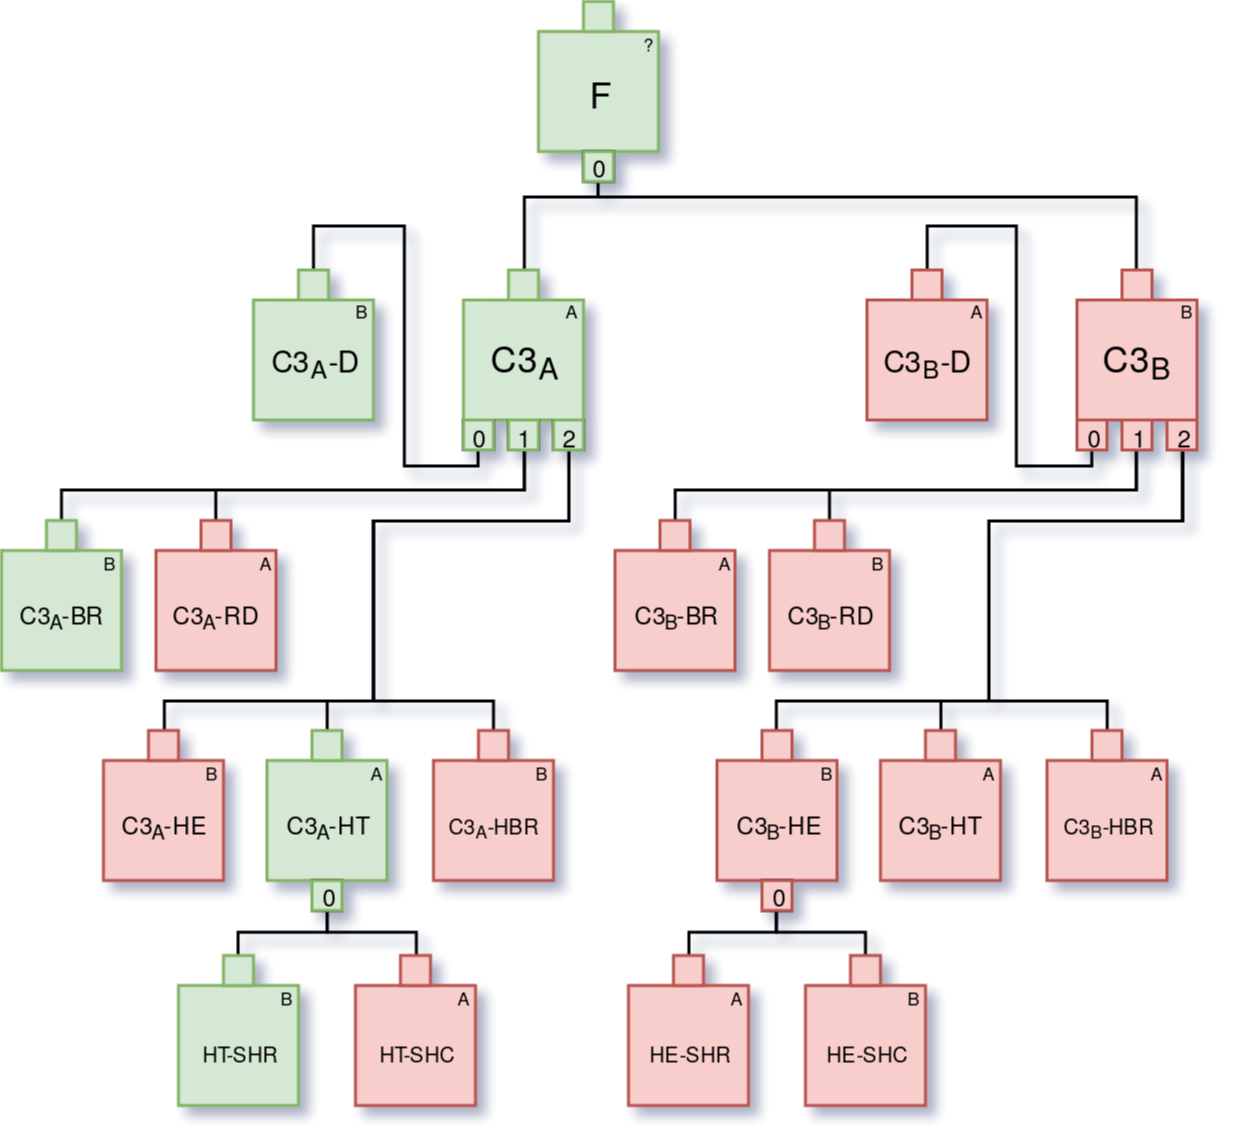
\includegraphics[width=0.80\textwidth]{background/images/payment_channel_htlc_revoked_bob.png}
	\caption{Same as figure \ref{fig:pc-htlc-revoked-alice}, but a different path}
	\label{fig:pc-htlc-revoked-bob}
\end{figure}
